% Options for packages loaded elsewhere
% Options for packages loaded elsewhere
\PassOptionsToPackage{unicode}{hyperref}
\PassOptionsToPackage{hyphens}{url}
\PassOptionsToPackage{dvipsnames,svgnames,x11names}{xcolor}
%
\documentclass[
  british,
  a4paper,
]{article}
\usepackage{xcolor}
\usepackage{amsmath,amssymb}
\setcounter{secnumdepth}{-\maxdimen} % remove section numbering
\usepackage{iftex}
\ifPDFTeX
  \usepackage[T1]{fontenc}
  \usepackage[utf8]{inputenc}
  \usepackage{textcomp} % provide euro and other symbols
\else % if luatex or xetex
  \usepackage{unicode-math} % this also loads fontspec
  \defaultfontfeatures{Scale=MatchLowercase}
  \defaultfontfeatures[\rmfamily]{Ligatures=TeX,Scale=1}
\fi
\usepackage{lmodern}
\ifPDFTeX\else
  % xetex/luatex font selection
\fi
% Use upquote if available, for straight quotes in verbatim environments
\IfFileExists{upquote.sty}{\usepackage{upquote}}{}
\IfFileExists{microtype.sty}{% use microtype if available
  \usepackage[]{microtype}
  \UseMicrotypeSet[protrusion]{basicmath} % disable protrusion for tt fonts
}{}
\makeatletter
\@ifundefined{KOMAClassName}{% if non-KOMA class
  \IfFileExists{parskip.sty}{%
    \usepackage{parskip}
  }{% else
    \setlength{\parindent}{0pt}
    \setlength{\parskip}{6pt plus 2pt minus 1pt}}
}{% if KOMA class
  \KOMAoptions{parskip=half}}
\makeatother
% Make \paragraph and \subparagraph free-standing
\makeatletter
\ifx\paragraph\undefined\else
  \let\oldparagraph\paragraph
  \renewcommand{\paragraph}{
    \@ifstar
      \xxxParagraphStar
      \xxxParagraphNoStar
  }
  \newcommand{\xxxParagraphStar}[1]{\oldparagraph*{#1}\mbox{}}
  \newcommand{\xxxParagraphNoStar}[1]{\oldparagraph{#1}\mbox{}}
\fi
\ifx\subparagraph\undefined\else
  \let\oldsubparagraph\subparagraph
  \renewcommand{\subparagraph}{
    \@ifstar
      \xxxSubParagraphStar
      \xxxSubParagraphNoStar
  }
  \newcommand{\xxxSubParagraphStar}[1]{\oldsubparagraph*{#1}\mbox{}}
  \newcommand{\xxxSubParagraphNoStar}[1]{\oldsubparagraph{#1}\mbox{}}
\fi
\makeatother


\usepackage{longtable,booktabs,array}
\newcounter{none} % for unnumbered tables
\usepackage{calc} % for calculating minipage widths
% Correct order of tables after \paragraph or \subparagraph
\usepackage{etoolbox}
\makeatletter
\patchcmd\longtable{\par}{\if@noskipsec\mbox{}\fi\par}{}{}
\makeatother
% Allow footnotes in longtable head/foot
\IfFileExists{footnotehyper.sty}{\usepackage{footnotehyper}}{\usepackage{footnote}}
\makesavenoteenv{longtable}
\usepackage{graphicx}
\makeatletter
\newsavebox\pandoc@box
\newcommand*\pandocbounded[1]{% scales image to fit in text height/width
  \sbox\pandoc@box{#1}%
  \Gscale@div\@tempa{\textheight}{\dimexpr\ht\pandoc@box+\dp\pandoc@box\relax}%
  \Gscale@div\@tempb{\linewidth}{\wd\pandoc@box}%
  \ifdim\@tempb\p@<\@tempa\p@\let\@tempa\@tempb\fi% select the smaller of both
  \ifdim\@tempa\p@<\p@\scalebox{\@tempa}{\usebox\pandoc@box}%
  \else\usebox{\pandoc@box}%
  \fi%
}
% Set default figure placement to htbp
\def\fps@figure{htbp}
\makeatother



\ifLuaTeX
\usepackage[bidi=basic,shorthands=off]{babel}
\else
\usepackage[bidi=default,shorthands=off]{babel}
\fi
\ifLuaTeX
  \usepackage{selnolig} % disable illegal ligatures
\fi


\setlength{\emergencystretch}{3em} % prevent overfull lines

\providecommand{\tightlist}{%
  \setlength{\itemsep}{0pt}\setlength{\parskip}{0pt}}



 


\makeatletter
\@ifpackageloaded{tcolorbox}{}{\usepackage[skins,breakable]{tcolorbox}}
\@ifpackageloaded{fontawesome5}{}{\usepackage{fontawesome5}}
\definecolor{quarto-callout-color}{HTML}{909090}
\definecolor{quarto-callout-note-color}{HTML}{0758E5}
\definecolor{quarto-callout-important-color}{HTML}{CC1914}
\definecolor{quarto-callout-warning-color}{HTML}{EB9113}
\definecolor{quarto-callout-tip-color}{HTML}{00A047}
\definecolor{quarto-callout-caution-color}{HTML}{FC5300}
\definecolor{quarto-callout-color-frame}{HTML}{acacac}
\definecolor{quarto-callout-note-color-frame}{HTML}{4582ec}
\definecolor{quarto-callout-important-color-frame}{HTML}{d9534f}
\definecolor{quarto-callout-warning-color-frame}{HTML}{f0ad4e}
\definecolor{quarto-callout-tip-color-frame}{HTML}{02b875}
\definecolor{quarto-callout-caution-color-frame}{HTML}{fd7e14}
\makeatother
\makeatletter
\@ifpackageloaded{caption}{}{\usepackage{caption}}
\AtBeginDocument{%
\ifdefined\contentsname
  \renewcommand*\contentsname{Table of contents}
\else
  \newcommand\contentsname{Table of contents}
\fi
\ifdefined\listfigurename
  \renewcommand*\listfigurename{List of Figures}
\else
  \newcommand\listfigurename{List of Figures}
\fi
\ifdefined\listtablename
  \renewcommand*\listtablename{List of Tables}
\else
  \newcommand\listtablename{List of Tables}
\fi
\ifdefined\figurename
  \renewcommand*\figurename{Figure}
\else
  \newcommand\figurename{Figure}
\fi
\ifdefined\tablename
  \renewcommand*\tablename{Table}
\else
  \newcommand\tablename{Table}
\fi
}
\@ifpackageloaded{float}{}{\usepackage{float}}
\floatstyle{ruled}
\@ifundefined{c@chapter}{\newfloat{codelisting}{h}{lop}}{\newfloat{codelisting}{h}{lop}[chapter]}
\floatname{codelisting}{Listing}
\newcommand*\listoflistings{\listof{codelisting}{List of Listings}}
\makeatother
\makeatletter
\makeatother
\makeatletter
\@ifpackageloaded{caption}{}{\usepackage{caption}}
\@ifpackageloaded{subcaption}{}{\usepackage{subcaption}}
\makeatother
\usepackage{bookmark}
\IfFileExists{xurl.sty}{\usepackage{xurl}}{} % add URL line breaks if available
\urlstyle{same}
% fallback for those not using the hyperref driver hyperxmp:
\makeatletter
\@ifundefined{xmpquote}{\newcommand{\xmpquote}[1]{#1}}{}
\makeatother
\hypersetup{
  pdftitle={A working map of macroeconomic model families},
  pdfauthor={Carlos Galindo},
  pdflang={en-GB},
  colorlinks=true,
  linkcolor={blue},
  filecolor={Maroon},
  citecolor={Blue},
  urlcolor={Blue},
  pdfcreator={LaTeX via pandoc}}


\title{A working map of macroeconomic model families}
\usepackage{etoolbox}
\makeatletter
\providecommand{\subtitle}[1]{% add subtitle to \maketitle
  \apptocmd{\@title}{\par {\large #1 \par}}{}{}
}
\makeatother
\subtitle{From the three-equation model to DSGE, and what each says
about exchange rates}
\author{Carlos Galindo}
\date{}
\begin{document}
\maketitle


\begin{tcolorbox}[enhanced jigsaw, arc=.35mm, bottomrule=.15mm, breakable, colback=white, colframe=quarto-callout-note-color-frame, left=2mm, leftrule=.75mm, opacityback=0, rightrule=.15mm, toprule=.15mm]

\vspace{-3mm}\textbf{At a glance}\vspace{3mm}

\begin{itemize}
\tightlist
\item
  \textbf{Question.} What does each major family of macroeconomic model
  assume, what does it let you say about a policy shock, and where do
  the families disagree?
\item
  \textbf{Approach.} Work through the families in order of complexity,
  from the three-equation model and quarterly projection models for
  small open economies to New Keynesian and DSGE models, and anchor the
  exchange-rate side in a self-built base of over 80 papers.
\item
  \textbf{Finding.} The families are best read as one ladder: each adds
  one structural ingredient (expectations, an open economy, optimising
  agents) and each ingredient changes which shocks matter and how fast
  they fade.
\item
  \textbf{Why it matters.} A forecaster or policy analyst who knows what
  each model assumes can say when a simple tool is enough and when it is
  misleading.
\end{itemize}

\end{tcolorbox}

\subsection{The question}\label{the-question}

Macroeconomists talk about ``the model'' as if there were one. There are
several, built for different purposes, and the choice among them often
decides the answer. A three-equation model can tell a central bank in a
few lines what happens to inflation if rates rise. A fully micro-founded
model can say whether a policy is welfare-improving, but only at the
price of heavy machinery. A small open economy adds a further wrinkle:
the exchange rate moves with expectations and with foreign interest
rates, and it can jump.

This project builds a working map of those families. The aim is not a
new model but a clear understanding of how the existing ones relate:
which assumptions are shared, which are added at each step, and which
empirical regularities each can or cannot reproduce. The reader it
serves is anyone who has to choose a model for a forecast, a scenario or
a policy discussion, and wants to know what that choice quietly assumes.

\subsection{Approach}\label{approach}

The work proceeds in four stages, each building on the last.

\textbf{The three-equation model.} The starting point is a closed
economy described by a demand curve linking output to the real interest
rate, a Phillips curve linking inflation to slack, and a policy rule
setting the interest rate in response to inflation and the output gap.
The compact version used here is written in continuous time, with a
decaying demand shock. Output feeds unemployment through a stable
output--unemployment relationship, unemployment feeds inflation, and the
policy rate closes the loop by feeding back into output. The key
analytic question is stability: the loop is self-correcting only if the
policy response to inflation is sufficiently strong, which is the
familiar requirement that the rate rises by more than one-for-one with
inflation.

\textbf{Quarterly projection models for small open economies.} The next
step adds an exchange rate, foreign variables and forward-looking
expectations. This is the structure many central banks use for routine
forecasting: a few behavioural equations, gaps defined against trends,
and an explicit policy rule. A central part of the study was a
derivation showing how a model with rational expectations can, under
stated conditions, be transformed into an equivalent vector
autoregression. That matters because it connects a structural model,
whose parameters have economic meaning, to a reduced form that can be
estimated and checked against data. The derivation also sets out the
minimum set of inputs needed to build such a system, the conditions for
a unique stable solution, and the role of eigenvalues in judging
determinacy.

\textbf{New Keynesian and DSGE models.} The third step makes households
and firms optimise. Demand and the Phillips curve are then derived
rather than assumed, expectations enter both, and shocks to technology,
preferences and policy are specified explicitly. A basic real business
cycle model served as the benchmark: solved to first order, simulated
over a long sample after discarding a burn-in, and used to produce
impulse responses over twenty periods. It is the simplest case in which
the whole workflow, from steady state through solution to simulation,
can be checked end to end.

\textbf{Exchange-rate overshooting and interest parity.} The fourth
strand follows one question across all the families: how does the
exchange rate respond to a monetary shock? The overshooting model gives
a sharp answer. Prices are sticky in the short run but asset markets
clear at once, capital is perfectly mobile, so interest parity holds and
expectations are rational. A monetary expansion then depreciates the
currency by more than its long-run amount, and the currency appreciates
back as prices catch up. To test this against the evidence, a structured
base of over 80 papers was assembled and converted into a searchable,
machine-readable form, with a survey of the interest parity literature
drawn from it.

How the work was checked: each model was written out in full, solved,
and compared with the qualitative behaviour the literature reports
(stability conditions, the sign and timing of responses, the size of
overshooting relative to the long-run move). Summaries drawn from the
paper base were treated as drafts and cross-read against the source
papers.

\subsection{What the work shows}\label{what-the-work-shows}

\subsubsection{Policy strength decides whether shocks
fade}\label{policy-strength-decides-whether-shocks-fade}

In the three-equation model a temporary demand shock raises output,
which lowers unemployment, which pushes inflation up, which prompts the
policy rate to rise and pull output back. How quickly this happens
depends on how hard the rule responds. A weak response lets inflation
drift for a long time; a strong one removes it quickly, at the cost of
larger swings in the policy rate. The figure shows the shape of this
trade-off in a discrete-time version with illustrative parameters.

\begin{figure}

\centering{

\pandocbounded{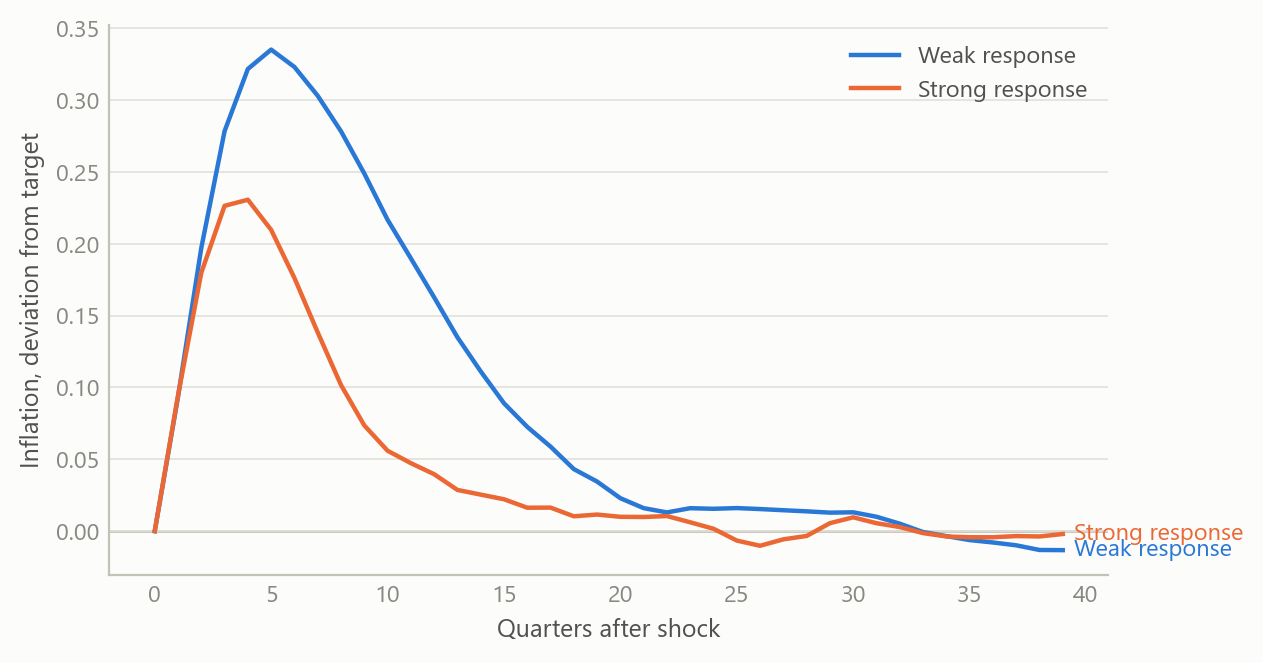
\includegraphics[keepaspectratio]{index_files/figure-latex/fig-three-eq-output-1.png}}

}

\caption{\label{fig-three-eq}Response of inflation to a temporary demand
shock under a weak and a strong policy response (simulated data).}

\end{figure}%

\subsubsection{The exchange rate overshoots, then
returns}\label{the-exchange-rate-overshoots-then-returns}

In the open-economy ladder, the exchange rate is the variable that
jumps. After an unexpected monetary expansion the currency depreciates
beyond its eventual level, while prices rise only slowly. The excess
depreciation is exactly what makes the interest differential offset
expected appreciation, so parity holds throughout. The figure shows both
paths.

\begin{figure}

\centering{

\pandocbounded{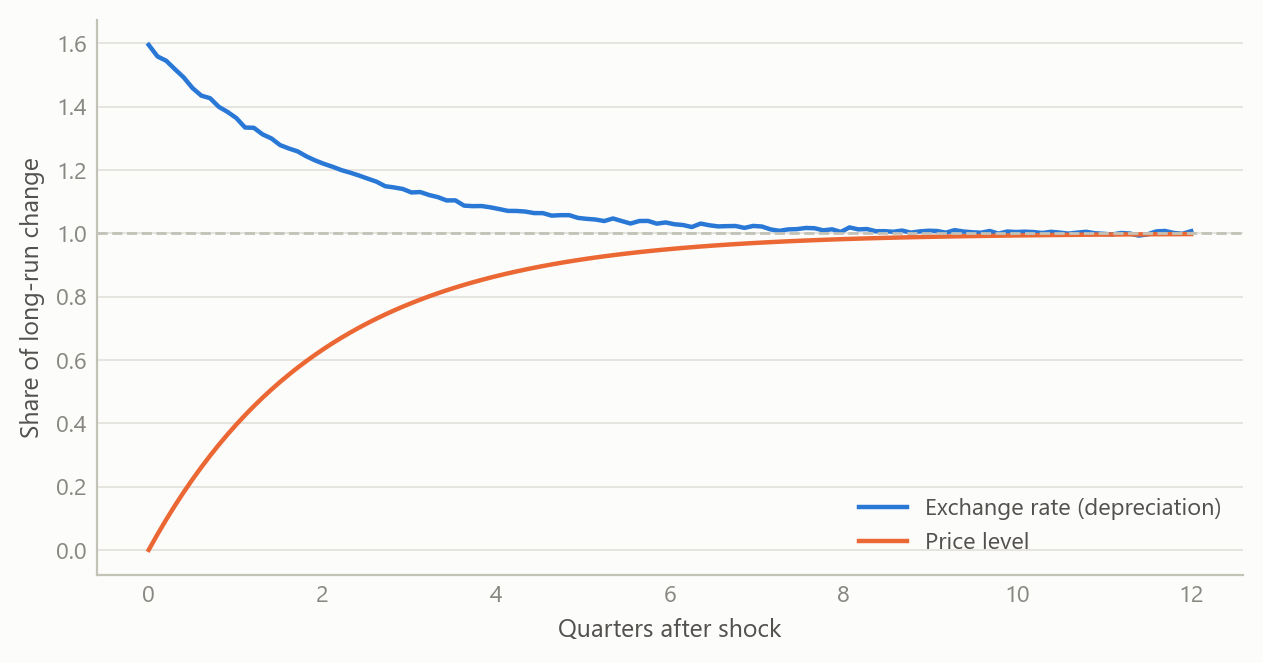
\includegraphics[keepaspectratio]{index_files/figure-latex/fig-overshoot-output-1.png}}

}

\caption{\label{fig-overshoot}Exchange rate and price level after an
unexpected monetary expansion, as a share of the long-run change
(simulated data).}

\end{figure}%

\subsubsection{Interest parity fails in simple tests, and the failure
shrinks under
scrutiny}\label{interest-parity-fails-in-simple-tests-and-the-failure-shrinks-under-scrutiny}

The simple parity condition says the expected change in the exchange
rate equals the interest differential. The standard test regresses the
realised change on the differential, where parity implies a slope of
one. In practice the slope is often well below one and sometimes
negative, the so-called forward premium puzzle. The survey drawn from
the paper base sets out six candidate explanations: time-varying risk
premia, market microstructure, investor sentiment, measurement and
small-sample bias, rare-disaster risk, and carry-trade dynamics with
limits to arbitrage.

The most useful single finding concerns publication bias. A published
meta-analysis of 3,643 estimates from 91 articles reports that, after
correcting for selective publication, the corrected slope is about 0.31
for developed markets and about 0.98 for emerging markets. In other
words, the puzzle is real but smaller than the raw literature suggests
for developed economies, and close to absent for emerging ones. The
figure reproduces the logic with simulated estimates: when small,
imprecise studies with low slopes are more likely to be published, the
published average falls below the truth.

\begin{figure}

\centering{

\pandocbounded{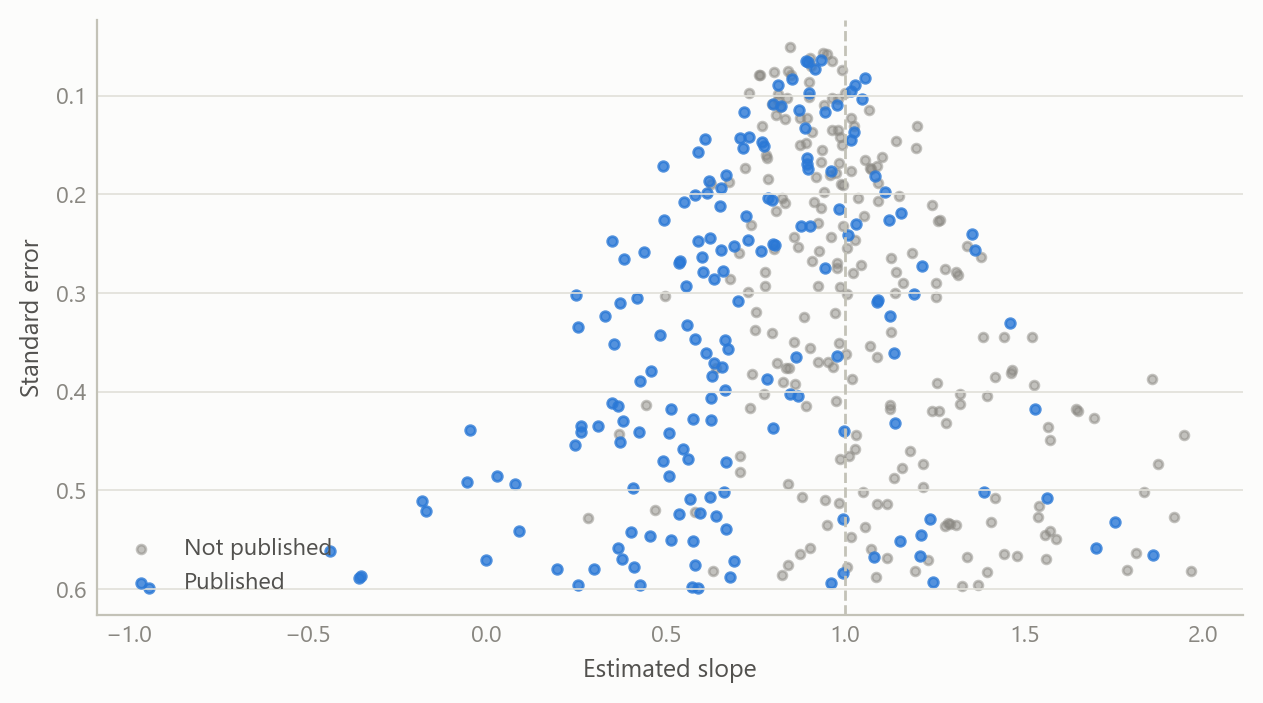
\includegraphics[keepaspectratio]{index_files/figure-latex/fig-bias-output-1.png}}

}

\caption{\label{fig-bias}Simulated study estimates of the parity slope:
all studies versus the subset more likely to be published (simulated
data).}

\end{figure}%

\subsubsection{What each rung adds}\label{what-each-rung-adds}

The table summarises what each family adds and what it costs.

{\def\LTcaptype{none} % do not increment counter
\begin{longtable}[]{@{}
  >{\raggedright\arraybackslash}p{(\linewidth - 6\tabcolsep) * \real{0.2500}}
  >{\raggedright\arraybackslash}p{(\linewidth - 6\tabcolsep) * \real{0.2500}}
  >{\raggedright\arraybackslash}p{(\linewidth - 6\tabcolsep) * \real{0.2500}}
  >{\raggedright\arraybackslash}p{(\linewidth - 6\tabcolsep) * \real{0.2500}}@{}}
\toprule\noalign{}
\begin{minipage}[b]{\linewidth}\raggedright
Family
\end{minipage} & \begin{minipage}[b]{\linewidth}\raggedright
What is added
\end{minipage} & \begin{minipage}[b]{\linewidth}\raggedright
What it can say
\end{minipage} & \begin{minipage}[b]{\linewidth}\raggedright
Main cost
\end{minipage} \\
\midrule\noalign{}
\endhead
\bottomrule\noalign{}
\endlastfoot
Three-equation model & Demand, Phillips curve, policy rule & Stability
and policy strength & Closed economy, ad hoc expectations \\
Quarterly projection model & Exchange rate, foreign block,
forward-looking terms & Routine forecasts and scenarios & Many gaps to
be measured \\
New Keynesian / DSGE & Optimising agents, explicit shocks & Welfare and
structural shocks & Heavy solution and estimation \\
Overshooting and parity & Sticky prices, mobile capital & Exchange-rate
dynamics & Parity fails in simple tests \\
\end{longtable}
}

\subsection{Insights}\label{insights}

\begin{itemize}
\tightlist
\item
  \textbf{Stability is a property of the policy rule, not only of the
  economy.} The same shock fades or lingers depending on how strongly
  the rule responds to inflation.
\item
  \textbf{Models are nested.} The richer models reduce to the simpler
  ones under restrictions, so the simple ones are a sound first read,
  not a rival.
\item
  \textbf{A structural model can be turned into an estimable reduced
  form.} Showing the equivalent vector autoregression, and the
  conditions under which it exists, is what links theory to testing.
\item
  \textbf{The exchange rate is the hard variable.} Overshooting is
  elegant, parity is its cornerstone, and parity is the part the data
  most often reject.
\item
  \textbf{Literature evidence needs bias correction.} Weighing a puzzle
  by the raw count of published estimates overstates it.
\end{itemize}

\subsection{Scope and next steps}\label{scope-and-next-steps}

This is a study of model families, not an estimate of any one economy.
The models were solved and compared for qualitative behaviour; none was
taken through a full estimation against a national data set here, and
the figures are illustrations, not results. The paper base was converted
automatically, and a minority of entries could not be retrieved in full,
so surveys drawn from it lean on the papers that were. The natural next
steps are to calibrate a small open economy projection model to a chosen
country, estimate the implied reduced form, and compare forecast
performance of the rungs out of sample.

\subsection{About the evidence}\label{about-the-evidence}

The work was done during a career break (from 2024, with the material
here dated 2025) as self-directed study, and combines written
derivations, solved model runs and a structured base of over 80 papers.
The one external number reported (the meta-analysis figures) comes from
that paper base. Everything plotted is simulated.

Figures and tables marked \emph{simulated} are generated from simulated
data built to share the structure of the analysis (its variables,
horizons and frequencies). They show how each method works and what its
output looks like. Results stated in the text, and figures that give a
source, are the project's own. Methods are described at the level of a
methods section. Code and data pipelines are not reproduced here.




\end{document}
